Estas notas van dirigidas mayormente a estudiantes de Alto Rendimiento que se preparan con esmero para enfrentar las diferentes competencias convocadas por las matemáticas.

$1\hspace{-0.05cm}\cdot\hspace{-0.05cm}\text{-}$ En todo $\triangle$ se cumple que: $a+b>c$, $b+c>a$, $c+a>b \longrightarrow$ Teorema de la desigualdad triangular.

$2\hspace{-0.05cm}\cdot\hspace{-0.05cm}\text{-}$ En todo $\triangle$ se cumple que: el segmento que une los puntos medios de dos de sus lados es paralelo al tercero y mide su mitad $\longrightarrow$ Teorema de la paralela media de un $\triangle$.

$3\hspace{-0.05cm}\cdot\hspace{-0.05cm}\text{-}$ Si dos bisectrices de un $\triangle$ tienen igual longitud $\Longrightarrow$ el $\triangle$ es isósceles $\longrightarrow$ Teorema de Steiner

$4\hspace{-0.05cm}\cdot\hspace{-0.05cm}\text{-}$ La suma de las distancias desde un punto interior de un $\triangle$ equilátero a los lados del $\triangle$ es $=$ a la longitud de su altura $\longrightarrow$ Teorema de Viviani

$5\hspace{-0.05cm}\cdot\hspace{-0.05cm}\text{-}$ Si sobre los lados $\overline{AB}$ y $\overline{AC}$ de un $\triangle ABC$ se construyen, por fuera, los $\triangle$ equiláteros $ABC'$ y $CAB' \Longrightarrow \overline{BB'} = \overline{CC'}$

$6\hspace{-0.05cm}\cdot\hspace{-0.05cm}\text{-}$ Si $G$ es el baricentro de un $\triangle ABC$ y por $G$ se traza una recta que corte a los 3 lados $\Longrightarrow \overline{AX} + \overline{BZ} = \overline{CY}$, siendo $\overline{AX}$, $\overline{BZ}$ y $\overline{CY}$ perpendiculares desde $A$, $B$, $C$ a la recta.

$7\hspace{-0.05cm}\cdot\hspace{-0.05cm}\text{-}$ Las proyecciones de un punto de una circunferencia sobre los lados de un $\triangle$ inscrito en dicha circunferencia determinan una recta $\longrightarrow$ Recta de Simpson.

$8\hspace{-0.05cm}\cdot\hspace{-0.05cm}\text{-}$ Circunferencia de los 9 puntos $\longrightarrow$ Es la que pasa por los puntos medios de cada lado, los pies de las alturas y los puntos medios de los segmentos que unen los vértices al ortocentro de un $\triangle$. El centro de esta circunferencia es el punto medio desde el ortocentro al centro de la circunferencia circunscrita.

$9\hspace{-0.05cm}\cdot\hspace{-0.05cm}\text{-}$ Triángulo pedal $\longrightarrow$ Es el $\triangle$ determinado por los pies de las alturas de un $\triangle$. El ortocentro del $\triangle$ coincide con el incentro del $\triangle$ pedal.

$ 10\hspace{-0.05cm}\cdot\hspace{-0.05cm}\text{-} $ Teorema de Stewart: Sea $\overline{AD} $ una ceviana cualquiera...

\noindent\parbox[][][t]{.4\linewidth}{
    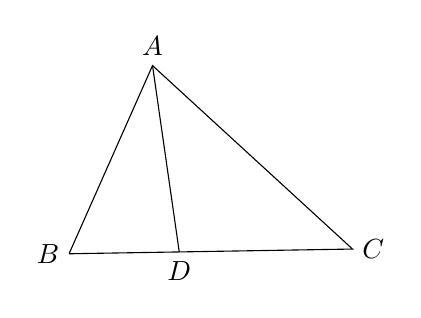
\begin{tikzpicture}
      \coordinate [label=left:$B$] (B) at (0,0);
      \coordinate [label=right:$C$] (C) at (3.6,0.06);
      \coordinate [label=above:$A$] (A) at (1.06,2.39);
      \coordinate [label=below:$D$] (D) at (1.4,0.02);
      \draw (B) -- (C) -- (A) -- (B);
      \draw (A) -- (D);
    \end{tikzpicture}
}
\parbox[][][t]{.05\linewidth}{\hspace{.05\linewidth}}
\parbox[][][t]{.55\linewidth}{
 $\overline{AB}^2\cdot\overline{DC} + \overline{AC}^2\cdot\overline{BD} = \overline{AD}^2\cdot\overline{BC} + \overline{BD}\cdot\overline{DC}\cdot\overline{BC}$
 
 \vspace{0.4cm}
 
 Para su demostración, trace la altura desde $A$ y aplique reiteradas veces el teorema de Pitágoras
 
}

\vspace{0.4cm}

$ 11\hspace{-0.05cm}\cdot\hspace{-0.05cm}\text{-} $  ???? bisectriz interior y exterior de un $\triangle$

\noindent\parbox[][][t]{.32\linewidth}{
    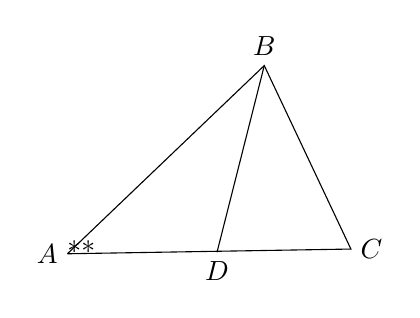
\begin{tikzpicture}
      \coordinate [label=left:$A$] (A) at (0,0);
      \coordinate [label=right:$C$] (C) at (3.6,0.06);
      \coordinate [label=above:$B$] (B) at (2.5,2.39);
      \coordinate [label=below:$D$] (D) at (1.9,0.02);
      
      \draw (A) -- (C) -- (B) -- (A);
      \draw (B) -- (D);
      \tkzLabelAngle[pos=0.5](A,B,D){$*$};
      \tkzLabelAngle[pos=0.5](D,B,C){$*$};
    \end{tikzpicture}
}
\parbox[][][t]{.15\linewidth}{$\dfrac{\overline{AB}}{\overline{BC}}=\dfrac{\overline{AD}}{\overline{DC}}$}
\parbox[][][t]{.53\linewidth}{
 \begin{tikzpicture}
      \coordinate [label=left:$A$] (A) at (0,0);
      \coordinate [label=above:$B$] (B) at (3.68,1.82);
      \coordinate [label=below:$C$] (C) at (3.9,0);
      
      \coordinate [label=below:$D$] (D) at (7.05,0);
      \coordinate [label=left:] (E) at (4.75,2.35);
      \draw (A) -- (C) -- (B) -- (A);
      \draw (B) -- (D);
      \draw[dashed] (C) -- (D);
      \draw[dashed] (B) -- (E);
      \tkzLabelAngle[pos=0.5](C,B,D){$*$};
      \tkzLabelAngle[pos=0.4](D,B,E){$*$};
    \end{tikzpicture}
}


\newpage

$ 12\hspace{-0.05cm}\cdot\hspace{-0.05cm}\text{-} $  Teorema de Ceva y Menelao

\noindent\parbox[][][t]{.35\linewidth}{
    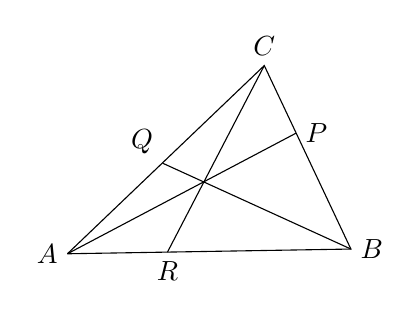
\begin{tikzpicture}
      \coordinate [label=left:$A$] (A) at (0,0);
      \coordinate [label=right:$B$] (B) at (3.6,0.06);
      \coordinate [label=above:$C$] (C) at (2.5,2.39);
      
      \coordinate [label=above left:$Q$] (Q) at (1.21,1.15);
      \coordinate [label=right:$P$] (P) at (2.9,1.53);
      \coordinate [label=below:$R$] (R) at (1.27,0.02);
      
      \draw (A) -- (B) -- (C) -- (A);
      \draw (A) -- (P);
      \draw (B) -- (Q);
      \draw (C) -- (R);
      
    \end{tikzpicture}
}
\parbox[][][t]{.2\linewidth}{$\dfrac{\overline{AR}}{\overline{RB}}\cdot\dfrac{\overline{BP}}{\overline{PC}}\cdot\dfrac{\overline{CQ}}{\overline{QA}}=1$}
\parbox[][][t]{.45\linewidth}{
    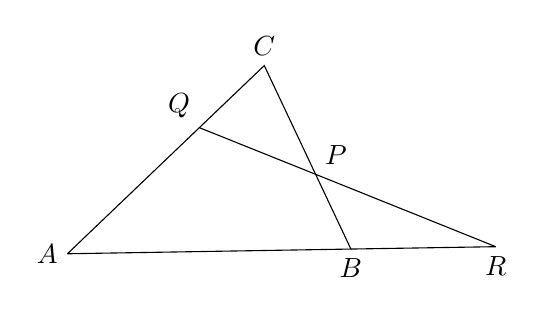
\begin{tikzpicture}
      \coordinate [label=left:$A$] (A) at (0,0);
      \coordinate [label=below:$B$] (B) at (3.6,0.06);
      \coordinate [label=above:$C$] (C) at (2.5,2.39);
      
      \coordinate [label=above left:$Q$] (Q) at (1.68,1.6);
      \coordinate [label=above right:$P$] (P) at (3.15,1.01);
      \coordinate [label=below:$R$] (R) at (5.44,0.09);
      
      \draw (A) -- (B) -- (C) -- (A);
      \draw (B) -- (R);
      \draw (Q) -- (P) -- (R);
      
      
    \end{tikzpicture}
}

 \vspace{0.4cm}
 
$ 13\hspace{-0.05cm}\cdot\hspace{-0.05cm}\text{-} $ Teorema de Pascal: En todo hexágono inscriptible sin lados opuestos paralelos, las intersecciones de los lados opuestos determinan 3 puntos alineados

$ 14\hspace{-0.05cm}\cdot\hspace{-0.05cm}\text{-} $ Desigualdad de Euler: $R \ge 2r$ con igualdad si el $\triangle$ es equilátero. $R \rightarrow $ circunradio, $r \rightarrow$ inradio

$ 15\hspace{-0.05cm}\cdot\hspace{-0.05cm}\text{-} $ Cálculo de áreas:
\begin{itemize}
    \item[-] $\triangle$ : $A = \dfrac{b\cdot h}{2}= \dfrac{a\cdot b \sen \gamma}{2} = \rho r = \dfrac{abc}{4R} = \sqrt{\rho(\rho-a)(\rho-b)(\rho-c)}$ (Herón)\vspace{0.4cm}\\
    $a$, $b$, $c$ lados del $\triangle$, $h \rightarrow$ altura del lado $b$\\
    $\gamma \rightarrow$ ángulo opuesto al lado $c$\\
    $\rho \rightarrow$ semiperímetro del $\triangle$
    
    \item[-] Cuadrilátero: $A = \dfrac{d_1 \cdot d_2}{2} \sen \sigma $\vspace{0.4cm}\\
    $d_1$, $d_2 \rightarrow$ diagonales, \hspace{0.5cm}$\sigma \rightarrow \measuredangle$ formado por las diagonales
\end{itemize}

$ 16\hspace{-0.05cm}\cdot\hspace{-0.05cm}\text{-} $  En todo paralelogramo la suma de los cuadrados de sus lados multiplicados por dos es $=$ a la suma de los cuadrados de sus diagonales.

$ 17\hspace{-0.05cm}\cdot\hspace{-0.05cm}\text{-} $ Teorema de Varignon: Al unir los 4 puntos medios de cada lado de un cuadrilátero se obtiene un paralelogramo.

\begin{center}
    \texttt{Algunos lemas necesarios}
\end{center}

$ 18\hspace{-0.05cm}\cdot\hspace{-0.05cm}\text{-} $  La distancia del circuncentro a uno de los lados de un $\triangle$ tiene la mitad de la longitud del segmento que une al ortocentro del $\triangle$ con el vértice opuesto al lado.

$ 19\hspace{-0.05cm}\cdot\hspace{-0.05cm}\text{-} $ Si $\overline{AB} \perp \overline{CD}$ en $N \Longrightarrow \overline{AC}^2 = \overline{AD}^2  = \overline{BC}^2 = \overline{BD}^2$

$ 20\hspace{-0.05cm}\cdot\hspace{-0.05cm}\text{-} $ Si $\overline{AA_1} \perp \overline{BB_1} \Longrightarrow a^2 + b^2 = 5c^2$, con $\overline{AA_1}$ mediana de $a$ y $\overline{BB_1}$ mediana de $b$ en un $\triangle ABC$ (Esto se prueba aplicando 19)

$ 21\hspace{-0.05cm}\cdot\hspace{-0.05cm}\text{-} $ Lema de Raví: En $\triangle ABC$, $I$ es el incentro, $P$, $Q$, $R$ puntos de tangencia del incírculo con los lados del $\triangle \Longrightarrow$

\noindent\parbox[][][t]{.35\linewidth}{
    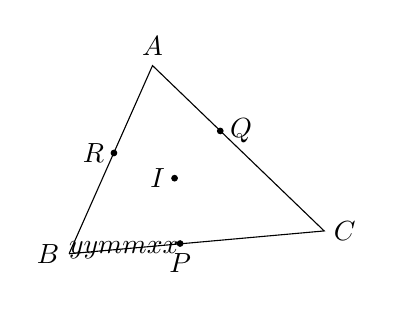
\begin{tikzpicture}
      \coordinate [label=left:$B$] (B) at (0,0);
      \coordinate [label=right:$C$] (C) at (3.24,0.29);
      \coordinate [label=above:$A$] (A) at (1.06,2.39);
      
      \coordinate [label=below:$P$] (P) at (1.41,0.13);
      \coordinate [label=right:$Q$] (Q) at (1.92,1.56);
      \coordinate [label=left:$R$] (R) at (0.57,1.28);
      
      \coordinate [label=left:$I$] (I) at (1.34,0.96);
      
      \draw (B) -- (C) -- (A) -- (B);
      
      \filldraw (I) circle[radius=1pt];
      \filldraw (P) circle[radius=1pt];
      \filldraw (Q) circle[radius=1pt];
      \filldraw (R) circle[radius=1pt];
      
      \tkzLabelSegment[left=1pt](B,R){$y$};  
      \tkzLabelSegment[below=1pt](B,P){$y$};
      
      \tkzLabelSegment[below=1pt](C,P){$m$};
      \tkzLabelSegment[right=1pt](C,Q){$m$};
      
      \tkzLabelSegment[left=1pt](A,R){$x$};
      \tkzLabelSegment[right=1pt](A,Q){$x$};
      
    \end{tikzpicture}
}
\parbox[][][t]{.05\linewidth}{\hspace{.05\linewidth}}
\parbox[][][t]{.6\linewidth}{
 $\overline{AR} = \overline{AQ} = x$, $\overline{BR} = \overline{BP} = y$, $\overline{CP} = \overline{CQ} = m$
 
\vspace{0.4cm}

 $\therefore a = y + m$, $b = m + x$, $c = x + y$

\vspace{0.4cm}
 
 $\Longrightarrow m = \dfrac{1}{2}(a+b-c)$, $y = \dfrac{1}{2}(c+b-b)$, $x = \dfrac{b+c-a}{2}$
}

\vspace{0.4cm}

$ 22\hspace{-0.05cm}\cdot\hspace{-0.05cm}\text{-} $ 


\noindent\parbox[][][t]{.49\linewidth}{
    \begin{tikzpicture}[scale=0.8]
      \coordinate [label=left:$T$] (T) at (-4,0);
      \coordinate [label=above right:$A$] (A) at (2.54,3.09);
      \coordinate [label=below:$B$] (B) at (1.51,-3.7);
      
      \coordinate [label=right:] (OI) at (-1.44,0);
      \coordinate [label=above:] (OE) at (0,0);
      
      \coordinate [label=right:$\omega$] (EI) at (1.12,0);
      \coordinate [label=left:$\Gamma$] (EE) at (4,0);
      
      \coordinate [label=above:$E$] (E) at (-1.77,2.54);
      \coordinate [label=below:$F$] (F) at (-2.26,-2.42);
      
      \coordinate [label=below:$A_1$] (A1) at (0.18,1.98);
      \coordinate [label=above:$B_1$] (B1) at (-0.47,-2.37);
      
      \tkzDrawCircle(OI,T);
      \tkzDrawCircle(OE,T);
      
      \draw (A) -- (T) -- (B) -- (A);
      \draw (A) -- (E);
      \draw (B) -- (F);
      
      \filldraw (E) circle[radius=1pt];
      \filldraw (F) circle[radius=1pt];
      \filldraw (A1) circle[radius=1pt];
      \filldraw (B1) circle[radius=1pt];
      
      
    \end{tikzpicture}
}
\parbox[][][t]{.51\linewidth}{
 Si $\omega$ y $\Gamma$ son dos circunferencias tangentes internas en $T$; $A$ y $B$ son puntos de $\Gamma$,\\$A_1 = \overline{TA} \bigcap \omega$ y $B_1 = \overline{TB} \bigcap \Gamma \Longrightarrow$
 
\vspace{0.4cm}
 
 \hspace{0.5cm}$\dfrac{\overline{TA}}{\overline{TB}}=\dfrac{\overline{AE}}{\overline{BF}}$ siendo $\overline{AE}$ y $\overline{BF}$ tangentes a $\omega$
 
\vspace{0.4cm}
 
 
 - Vea que $\overline{A_1B_1} \parallel \overline{AB}$\\y por potencia de un punto
 \begin{equation*}
     \begin{aligned}
      \overline{AE}^2 &= \overline{AA_1} \cdot \overline{AT}\\
      \overline{BF}^2 &= \overline{BB_1} \cdot \overline{BT}\text{, etc ...}
     \end{aligned}
 \end{equation*}
}

\vspace{0.4cm}

$ 23\hspace{-0.05cm}\cdot\hspace{-0.05cm}\text{-} $ 


\noindent\parbox[][][t]{.55\linewidth}{
    \begin{tikzpicture}[scale=0.8]
      \coordinate [label=above:$A$] (A) at (0.37,2.35);
      \coordinate [label=left:$B$] (B) at (-3.38,-1.4);
      \coordinate [label=right:$C$] (C) at (2.28,-1.4);
      
      \coordinate [label=below:$D$] (D) at (0,-1.4);
      \coordinate [label=right:$E$] (E) at (1.25,0.63);
      \coordinate [label=left:$F$] (F) at (-0.99,0.99);
      
      \coordinate [label=below left:$X$] (X) at (-1.1,-1.4);
      \coordinate [label=left:$Y$] (Y) at (3.78,-4.35);
      \coordinate [label=right:$Z$] (Z) at (-5.54,-3.58);
      
      
      \coordinate [label=below right:$T$] (T) at (0,1.4);
      \coordinate [label=right:$\sigma$] (O) at (0,0);
      
      \coordinate [label=right:$\sigma_a$] (Oa) at (-1.14,-7);
      
      \coordinate [label=right:] (P) at (-5.99, -4.01);
      \coordinate [label=right:] (Q) at (4.1,-4.98);
      
      \draw (B) -- (C) -- (A) -- (B);
      \draw (A) -- (P);
      \draw (A) -- (Q);
      \draw (T) -- (O) -- (D);
      \draw (A) -- (T) -- (X);
      \draw (Oa) -- (X);
      
      
      \filldraw (O) circle[radius=1.5pt];
      \filldraw (Z) circle[radius=1.5pt];
      \filldraw (Y) circle[radius=1.5pt];
      \filldraw (Oa) circle[radius=1.5pt];
    
    \tkzDrawCircle(O,T);
      
    \end{tikzpicture}
}
%\parbox[][][t]{.01\linewidth}{\hspace{.01\linewidth}}
\parbox[][][t]{.45\linewidth}{
 Si $D$, $E$, $F$ puntos de tangencia del incírculo de centro $\sigma$ en $\triangle ABC$. Si $\overline{DT}$ es diámetro; recta $\overrightarrow{AT}$ corta $BC$ en $X \Longrightarrow \overline{BD} = \overline{CX}$
 
 \vspace{0.4cm}
 
 Demostración:\vspace{0.1cm} \\$2 \overline{BD} = \overline{BC} + \overline{AB} - \overline{AC}$ por $21)$\\
 $= \overline{BF} + \overline{BZ} + \overline{XD}$\\
 $= \overline{FZ} + \overline{XD} = \overline{EY} + \overline{XD}$\\
 $= \overline{EC} + \overline{CY} + \overline{XD} = \overline{DC} + \overline{XC} + \overline{XD}$\\
 $= 2 \overline{CX}$
 
 \vspace{0.4cm}
 
 $Z$ y $Y$ puntos de tangencia del excírculo de $A$ con lados $\overrightarrow{AB}$ y $\overrightarrow{AC}$
}

\vspace{0.4cm}


\vspace{1cm}

24, 25, 26 ... pueden ser sugerencias de los amigos de la matemática.

